
\documentclass[svgnames]{beamer}

\mode<presentation> {
\usetheme{Warsaw}
}

\usepackage{graphicx}
\usepackage{booktabs}
\usepackage{listings}
\usepackage{color}
\usepackage[lofdepth,lotdepth]{subfig}
\usepackage{fontawesome}
\usepackage{hyperref}

\definecolor{codegreen}{rgb}{0,0.6,0}
\definecolor{codegray}{rgb}{0.5,0.5,0.5}
\definecolor{codepurple}{rgb}{0.58,0,0.82}
\definecolor{backcolour}{rgb}{0.95,0.95,0.92}


\lstdefinestyle{mystyle}{
    backgroundcolor=\color{backcolour},   
    commentstyle=\color{codegreen},
    keywordstyle=\color{magenta},
    numberstyle=\tiny\color{codegray},
    stringstyle=\color{codepurple},
    %basicstyle=\footnotesize,
    basicstyle=\scriptsize\ttfamily,
    breakatwhitespace=false,         
    breaklines=true,                 
    captionpos=b,                    
    keepspaces=true,                 
    numbers=left,                    
    numbersep=5pt,                  
    showspaces=false,                
    showstringspaces=false,
    showtabs=false,                  
    tabsize=2,
    language=bash
}

\lstset{style=mystyle}

% \newcommand{\SubItem}[1]{
%     {\setlength\itemindent{15pt} \item[-] #1}
% }

%------------
%	TITLE PAGE
%------------

\title[Version control, Git, GitHub and GitFlow]{Introduction to Git and GitFlow} 
\author{Criscely Luj\'{a}n \\ criscely.lujan@ird.fr \\ \and
Nicolas Barrier \\
nicolas.barrier@ird.fr}
\institute[Universit\'{e} Paris-Sud, UMR MARBEC]  
{Universit\'{e} Paris-Sud, UMR MARBEC \\ 
\medskip
\textit{criscely.lujan@ird.fr}
}
\author[shortname]{Criscely Luj\'{a}n\inst{1,2} \\ \vspace{-0.5em} \tiny \emph{\href{mailto:criscely.lujan@ird.fr}{criscely.lujan@ird.fr}} \normalsize \\ \vspace{1em}
                         \and Nicolas Barrier\inst{2}\\  \tiny \emph{\href{mailto:nicolas.barrier@ird.fr}{nicolas.barrier@ird.fr}}}
\institute[shortinst]{\inst{1} Universit\'{e} Paris-Sud, UMR MARBEC \and \inst{2} IRD, UMR MARBEC}

\date{April 11, 2019}

\begin{document}

%------------
\begin{frame}
    \titlepage 
    \begin{center}
        
\includegraphics[height=1.5cm]{img/logo_psud.jpg}
        \hspace{1em}
        
\includegraphics[height=1.5cm]{img/logo_marbec.png}
        \hspace{1em}
        
\includegraphics[height=1.5cm]{img/logo_ird.png}
    \end{center}
\end{frame}

\hypersetup{
    colorlinks=true,
    linkcolor=white,
    urlcolor=SteelBlue
}

\begin{frame}
    \frametitle{Version control}

    Also known as \textbf{revision control} or \textbf{source control}. \hfill \break

    ... ``\textit{is the management of changes:}

    \begin{itemize}
        \item \textit{documents
        \item computer programs
        \item large web sites
        \item other collections of information ... }''
    \end{itemize}
\end{frame}


\begin{frame}
    \frametitle{Why is important version control?}
    \begin{center}
        
\includegraphics[scale=0.29]{img/phd_comics.png}
    \end{center}
\end{frame}


\begin{frame}
    \frametitle{Why is important version control?}
    \begin{itemize}
        \item Storing \textbf{version} (properly). \hfill \break
        \item \textbf{Restoring} previous versions. \hfill \break
        \item \textbf{Collaborations} (networking). \hfill \break
        \item Save \textbf{time}. \hfill \break
    \end{itemize}
\end{frame}


\begin{frame}
    \frametitle{Version control software}
    \begin{center}
        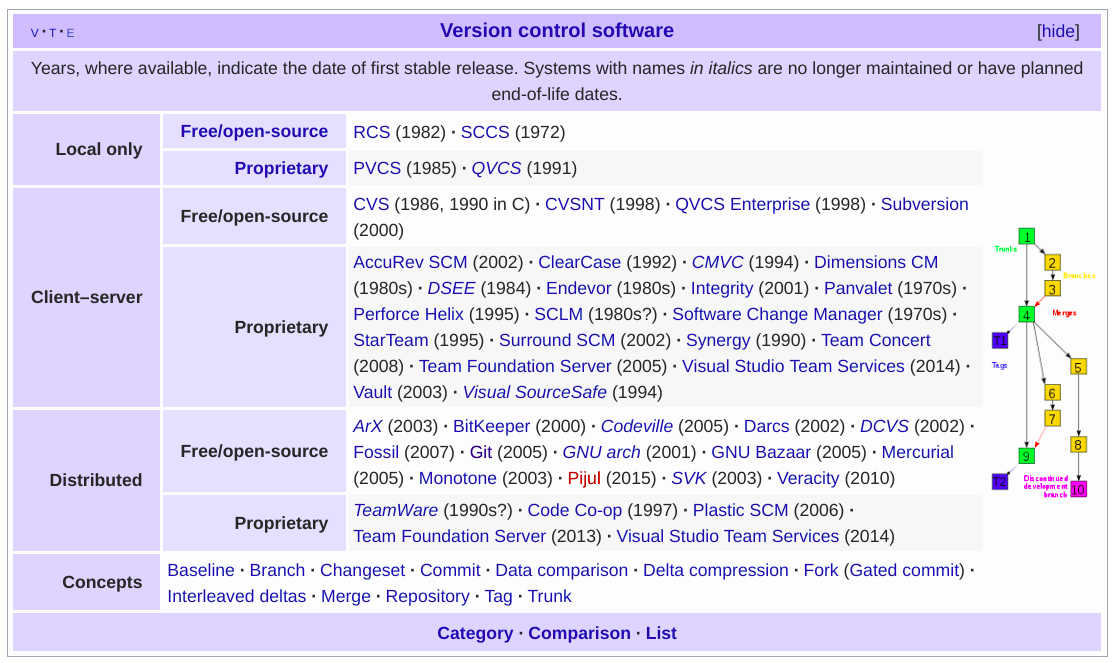
\includegraphics[scale=0.29]{img/controlVersion.png}
    \end{center}
\end{frame}


\begin{frame}
    \frametitle{What is Git?}

    \textbf{Git} is a distributed version control system for tracking changes in source code during the development of software.

    \hfill \break

    \begin{center}
        
\includegraphics[scale=0.07]{img/git_logo.png}
    \end{center}
\end{frame}


\begin{frame}
    \frametitle{Why use Git?}
    \begin{itemize}
        \item \textbf{Popular and successful}
            \begin{itemize}
                \item[$-$]{Active development}
                \item[$-$]{Fast}
                    \hfill \break
            \end{itemize}

        \item \textbf{Distributed}
            \begin{itemize}
                \item[$-$]{Work online and offline}
                \item[$-$]{Collaborate with large groups}
                    \hfill \break
            \end{itemize}

        \item \textbf{Tracks any type of file}
            \begin{itemize}
                \item[$-$]{Works best with text}
                    \hfill \break
            \end{itemize}

        \item \textbf{Branching}
            \begin{itemize}
                \item[$-$]{Smarter merges}
            \end{itemize}
    \end{itemize}
\end{frame}


\begin{frame}
    \frametitle{What is GitHub Inc.?}

    \begin{center}
        \textbf{GitHub} is a web-based hosting service for version control using \textbf{Git}.
    \end{center}

    \begin{center}
        
\includegraphics[scale=0.2]{img/github_logos.png}
    \end{center}
\end{frame}


\begin{frame}
    \frametitle{GitHub Inc.}
    \begin{itemize}
        \item Access to the control and collaboration features for every \textbf{project}. \hfill \break
        \item Work with public and private \textbf{repositories}. \hfill \break
        \item Develop a \textbf{networking}. \hfill \break
        \item \textbf{Plans} for enterprise, teams, pro and free accounts. \hfill \break
        \item Is the \textbf{largest} host of source code in the world! \emph{(28 million users, 57 million repositories (28 million public) - June 2018)}.
    \end{itemize}
\end{frame}


\begin{frame}
    \frametitle{Register a GitHub account}
    \begin{itemize}
        \item Register an account with \href{https://github.com/}{\faStar GitHub} is free! \hfill \break
        \item Free private repositories
            \begin{itemize}
                \item[$-$] Sudents, faculty, and educational / research staff: \href{https://education.github.com/}{\faStar GitHub Education}.
                \item[$-$] Official nonprofit organizations and charities: \href{https://github.com/nonprofit}{\faStar GitHub for Good}.
                    \hfill \break
            \end{itemize}
        \item Pay for private repositories
            \begin{itemize}
                \item[$-$] Individual cost is 7 dolars per month: \href{https://github.com/pricing}{\faStar GitHub Pricing}.
            \end{itemize}

    \end{itemize}
\end{frame}

\begin{frame}
    \frametitle{Institutionnal repository}

    GitHub is a private US company. There are also \emph{institutional} repositories on which Git can be used:

    \begin{itemize}
        \item{\href{https://sourcesup.renater.fr/}{Sourcesup}: this is a Renater platform (login possible from any French research institute or through CRU accounts)}
        \item{\href{https://forge.ifremer.fr/}{Forge Ifremer}: very close to SourceSup (Ifremer extranet account required)}
        \item{\href{gitlab.intranet.ird.fr}{IRD GitLab}: GitLab IRD platform (IRD account required).}
    \end{itemize}

    However, the projects hosted on these repositories may have less visibility...

\end{frame}


\begin{frame}
    \frametitle{Git clients}

    Git and Git client \textbf{are not} the same! Like R and RStudio is not the same thing!
    \hfill \break

    Git client:
    \begin{itemize}
        \item IDE (Integrated development environment)!
        \item Make the experience more pleasant providing a richer visual representation.
    \end{itemize}

    \hfill 

    Some Git clients:
    \begin{itemize}
        \item \href{https://www.sourcetreeapp.com/}{\faStar SourceTreen} 
        \item \href{https://www.gitkraken.com/}{\faStar GitKraken}
        \item \href{https://gitup.co/}{\faStar GitUp} 
        \item \href{https://www.syntevo.com/smartgit/}{\faStar SmartGit} 
        \item \href{https://git-cola.github.io/}{\faStar git-cola} 
        \item ... others... 
        \item \textbf{RStudio} 
    \end{itemize}
\end{frame}


\begin{frame}
    \frametitle{Git workflows} % Table of contents slide, comment this block out to remove it
    There are several ways to use GIT (we talk about \textbf{workflows}). 

    \begin{itemize}
        \item \emph{Centralized workflow}: one main branch, everyone commit in the same place.
        \item \emph{Feature Branch Workflow}: developments are made in dedicated branches (feature branches), which are regularly merged to the master one.
        \item \textbf{\textit{Gitflow Workflow}}: Strict branching model designed around the project release.
    \end{itemize}

    Source: \url{https://www.atlassian.com/git/tutorials/comparing-workflows}

\end{frame}

\begin{frame}{GitFlow branches}

    GitFlow workflow contains two main branches:
    \begin{itemize}
        \item{\emph{master:} official release history. Branch which is shared to the world!}
        \item{\emph{develop:} integration branch for features}
    \end{itemize}

    It also contains additional temporal branches:
    \begin{itemize}
        \item{\emph{feature}: feature branches (one for each new feature to add to the code)}
        \item{\emph{release}: branch created when enough features have been added (new version of the code)}
        \item{\emph{hotfix}: branch for maintenance and bug correction of the production release}
    \end{itemize}

\end{frame}

\begin{frame}{In summary...}

    \begin{center}
        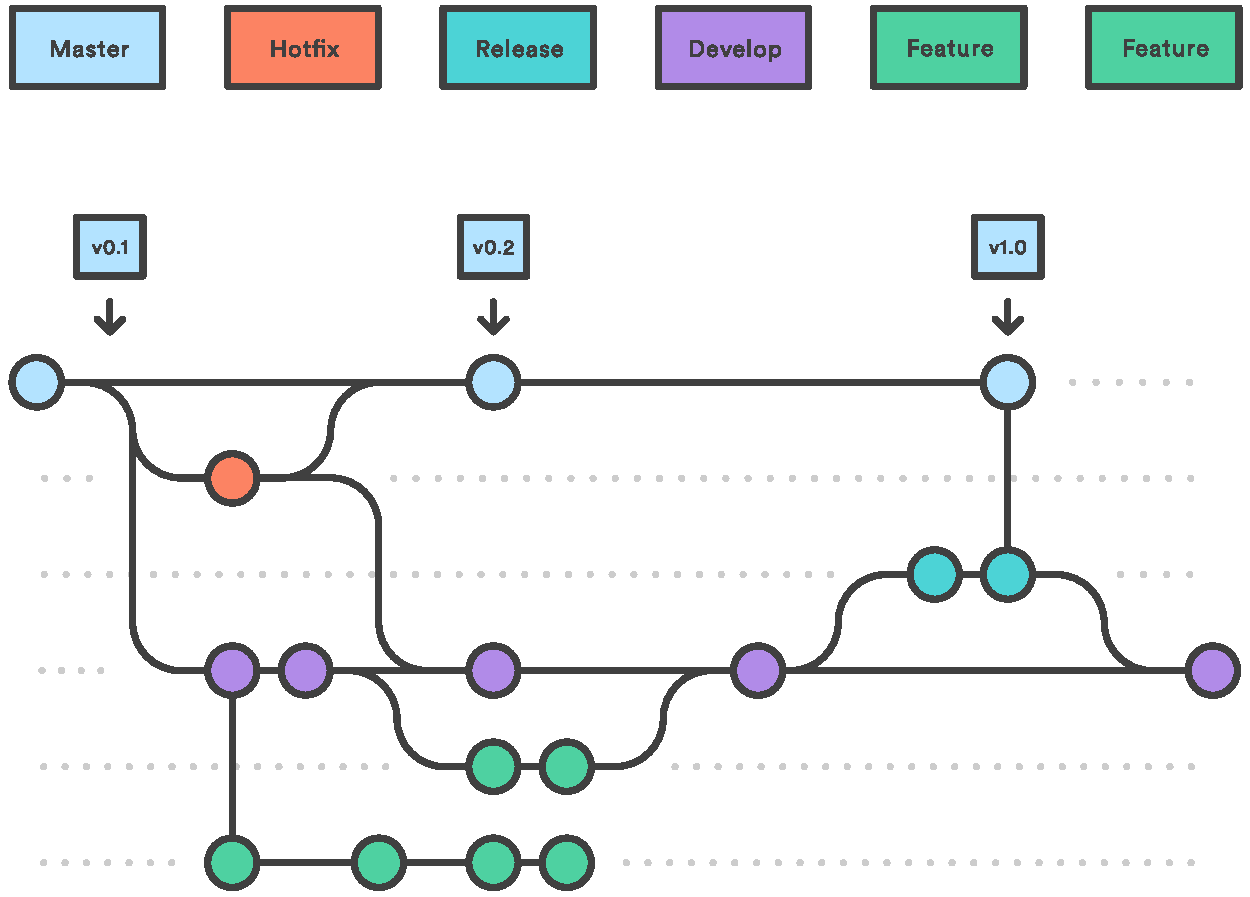
\includegraphics[scale=0.5]{05-_2_.pdf}    
    \end{center}

\end{frame}    

%\begin{frame}[fragile]{How it works in practice}
%
%    Install the GitFlow extension:
%
%    \begin{lstlisting}[language=bash]
%    sudo apt-get install git-flow
%    \end{lstlisting}
%
%    \vspace{1em}
%    Now, from your directory, initialize the GitFlow workflow:
%
%    \begin{lstlisting}[language=bash]
%    git flow init # create the develop branch
%    git push origin develop # push the develop branch to the repository
%    \end{lstlisting}
%
%\end{frame}
%
%\begin{frame}[fragile]{Creating new features}
%
%    \begin{lstlisting}
%    # recovers the latest develop branch
%    git pull origin develop
%
%    # create feature branch from develop and switch to it
%    git flow feature start my-feature 
%
%    # put the feature branch to the repo (not necessary)
%    git flow feature publish my-feature 
%
%    # edit/add files: new functionalities
%
%    # commit changes to the my-feature branch
%    git commit 
%
%    # merge my-feature branch with develop and remove it
%    # switch back to develop
%    git flow feature finish
%
%    # push updated develop branch
%    git push origin develop
%
%    # if conflict (someone has already pushed in develop)
%    git pull origin develop
%    git push origin develop
%    \end{lstlisting}
%
%\end{frame}
%
%\begin{frame}[fragile]{Creating a new release}
%
%    \begin{lstlisting}
%    # recovers the latest develop branch
%    git pull origin develop
%
%    # create a new release branch
%    git flow release start my-release
%
%    # put the release branch to the repo (not necessary)
%    git flow release publish my-release 
%
%    # edit/add files: bug fixes + documentation
%
%    # commit changes to the my-feature branch
%    git commit 
%
%    # finish the release
%    git flow release finish
%
%    # push updated develop/master and tags
%    git push origin --tags
%    git push origin develop
%    git push origin master
%    \end{lstlisting}
%\end{frame}
%
%\begin{frame}[fragile]
%    \frametitle{Creating hotfixes}
%    \begin{lstlisting}
%    # recovers the latest develop/master branches
%    git pull origin develop
%
%    # create a new hotfix branch from master
%    # name should be a version name (1.3.2 for instance)
%    git flow hotfix start hotfix-tag
%
%    # edit/add files: bug corrections
%
%    # commit changes to the hotfix-tag branch
%    git commit 
%
%    # finish the release
%    # merge hotfix branch to master/develop
%    git flow hotfix finish
%
%    # push updated develop/master and tags
%    git push origin --tags
%    git push origin develop
%    git push origin master
%    \end{lstlisting}
%\end{frame}

\begin{frame}
    \frametitle{References} % Table of contents slide, comment this block out to remove it

    \begin{itemize}
        \item \url{https://nvie.com/posts/a-successful-git-branching-model/}
        \item \url{https://www.atlassian.com/git/tutorials/comparing-workflows}
        \item \url{https://danielkummer.github.io/git-flow-cheatsheet/}
        \item \url{https://gist.github.com/JamesMGreene/cdd0ac49f90c987e45ac}
        \item \url{https://blog.xebia.fr/2018/03/28/gitflow-est-il-le-workflow-dont-jai-besoin/}
    \end{itemize}

\end{frame}



\end{document}
